% Configuration
\input{includes/config.tex}
%
\begin{document}
%
% Titlepage
\maketitle{Master Thesis}{International Software Systems Science}{Open‐Source Software Discovery and Vulnerability Analysis}{Rajendran, Hari Prashanth}{23.09.2021}
%
% TOCs
\begin{abstract}
In this technology era, most software developers and enterprises are bound to use open-source software components to reduce development efforts. Which also says 96\% of the applications used in enterprises is built through open-source software\cite{Gilad}. These \acs{OSS} components are shared with the help of portals like GitHub and GitLab. The main strength of the \acs{OSS} component, which is highly shareable and reusable, will be the most significant weakness. Due to its rising IT security threats, the security part is still being improved from the beginning of "shared code culture". An unsecured \acs{OSS} component may lead to substantial security threats. Most of the known security issues and threats are registered in vulnerability databases. There are few active vulnerability databases available in the market, and users can search \acs{OSS} components/software in the vulnerability database. 

This thesis builds an \acs{OSS} vulnerability scanning web application to extract and analyse the \acs{OSS} component used inside software projects. At the same time, the scanning takes place on the client-side due to the source code privacy of the user's software project. The automation of extracting the \acs{OSS} components is mandatory because a software project can consist of a lot of \acs{OSS} packages/libraries. The first step is to create an automated solution to extract the \acs{OSS} components. The \acs{OSS} scanner can scan most of the known software projects, and it is also built by considering the scalability of the software projects. The application will analyse the extracted components from the scanner to find the known vulnerability with the \acs{NVD} vulnerability database's help and retrieve all the known vulnerabilities of the \acs{OSS} components found in the project. Finally, the results will be analysed and converted into a simple pdf report to the end-user.
	
\end{abstract}
\newpage
\pagenumbering{Roman}
\tableofcontents
\newpage
\listoffigures
\newpage
\listoftables
\newpage
\lstlistoflistings
\newpage
\fancyhead[LO]{\footnotesize\sc\nouppercase{Abbreviations}}
%
% Abkürzungen
%
\section*{Abbreviations}
% In Klammern steht das längste Akronym!
\begin{acronym}[LSPI]
 \acro{DSG}{Distributed Systems Group}
 \acro{LSPI}{Lehrstuhl für Praktische Informatik}
 \acro{OSS}{Open-source Software}
 \acro{NVD}{National Vulnerability Database}
 \acro{CVE}{Common Vulnerabilities and Exposure}
 \acro{CVSS}{Common Vulnerability Scoring System}
 \acro{CERT/CC}{Computer Emergency Response Team Coordination Center}
\end{acronym}
\newpage
\fancyhead[LO]{\footnotesize\sc\nouppercase{\leftmark}}
\setcounter{page}{1}
\pagenumbering{arabic}
%
% Insert your chapters here
%
%
\section{Introduction}\label{sec:introduction}
%
Open-source software is a kind of computer program or application available to the public and has been developed collaboratively. It stands as free and open-source software (FOSS).
Open source development could be seen as a paradigm where the end-user can choose between varying shades of licensing types. It could also be seen as an economically prudent way for project developers to fund their work. The open-source movement was spurred by developers who wanted access to code because they wanted more control over what they created. Apart from the high benefits, the OSS also has many threats that make a drawback, but it can be resolved by taking precautions.
\subsection{Motivation}
Nowadays, firms and individuals use different forms of computer software running on other platforms, from a simple mobile application to a sophisticated distributed enterprise system. Even though the software is created using different methodologies based on a wide variety of technologies, still each has its advantages and disadvantages \cite{tur38}\cite{KaDaPeTu2014}. Software security is an essential concern in the software development process because not only to reduce the additional cost but also it can cause severe damage for developers or organizations \cite{fil2}. In some recent years, there have been many incidents in which software vulnerability imposed vital damage to companies and individuals. To make a clear idea of this issue, we have mentioned incidents that happened in recent years. A prominent example of an open-source software vulnerability is the Equifax breach in 2017, which exposed 145 million users' data due to outdated open-source software. The outcome of this incident relies openness because the same code has seen by all users, which includes the attackers\cite{WinNT}. Software vulnerabilities are imposed by the importance of the threats, which depend on the factors like exploitation complexity and attack-surface[8]. Likewise, there have been a lot of incidents before in companies and individuals have been affected by software vulnerability with significant damage \cite{tur38}. In addition, vulnerabilities are common and fundamental. Therefore, choosing software is essential to risk management for information security. Selecting software libraries with solid security features can reduce risk management to individuals or organizations. \acs{OSS} has been referred to as a potential answer for software security issues and vulnerabilities because most of the open-source software licenses give full access to any part of the code to examine and modify \cite{KeJaSa2005}.

\subsection{Problem Statement}
In general open-source software is used massively in modern Software Development, which says around 96\% of the application in the enterprise market uses open-source software\cite{Gilad}. Today standard components are not re-written; instead, they are shared as packages around the world. Open Source Portals like Github and Gitlab make it very easy to share those components. The advantage of this "Shared Code Culture" is also the most significant disadvantage because the whole Community and the components are constantly changing. Releases of components are often pushed daily if the project is active. However, if the community switches or the primary Authors leave, those projects depreciate very fast.

Moreover, due to rising IT security threats, a component can become insecure if not patched frequently. Whether an \acs{OSS} component will become critical also depends on the context where the component will be used. The context will define which actions need to be taken to use an \acs{OSS} component within the project. We propose to build a scanner to extract all the possible open-source software components and their dependencies from software projects and perform data analysis with the help of \acs{CVE} and \acs{NVD} to find the severity of each vulnerable component \cite{RaLo2016}. The first challenge for building this scanner will be scanning for open-source software components, which should happen on the client-side of the system due to the source code privacy of the projects.

Along with the scanning, the system should extract the open-source component meta information from various software projects by using the best text analysis approach. After the extraction of the open-source software components, the next challenge will be assessing the vulnerability and its security issues of each component by choosing a suitable predictive analysis model. The final output of this scanning will be a PDF report which gives precise detail of each open-source software component used inside the project.
\newpage
%
%
\section{Background}\label{sec:background}
%
\subsection{Open-source Software}
At a fundamental level, it is a software code available for all users to inspect, modify, copy and use in almost any way they choose. The first evolution of open-source software happened in the 1970s by Richard Stallman \cite{zh2011}. Commercial software often called proprietary software, also has additional licensing that further prohibits people from attempting to reverse engineer or modify this process. However, in open-source software, the source code is made available alongside the final executable program. It means any developers or programmers can modify the application to improve or customize it. The students also can study how the programs were written, and the programs can be easily copied and distributed over the internet with the help of cloud repositories \cite{MiViIa2013}. Supporters of open-source believe open collaboration allows the software to evolve via the contribution of many users. Also, they believe people should have the right to use their software in whatever way they want without licensing restrictions. The term open-source has made many impacts in computer science practising, whereas many technologies have generally been built and distributed by a permissive license. The open-source software focuses more on the term "free", which helps to build open and transparent software systems. It also helps to improve the project becoming reliable and scalable so that it will help the digital economy to grow \cite{MiViIa2013}.
%
\subsection{National Vulnerability Database}
The \acs{NVD} is one of the largest and most effective databases, which is used to report all known vulnerabilities for both commercial and open-source components. It was governed and operated under the US National Institute of Standards and Technology(NIST) from 2005. This organization is sponsored by the Department of Homeland Security's National Cybersecurity and Communications integration centre and Network Security deployment[13]. The information which has been provided by the \acs{NVD} database helps the developer or security member to help track the software security. The information from \acs{NVD} helps to analyze the software security vulnerability of an \acs{OSS} component. It also helps the user know what type of issues are in it and helps the user move further. A section of \acs{NVD} also provides information on \acs{CVE} as well as the information source, which is usually from the MITRE corporation \cite{TheNVD}. Figure~\ref{fig:vulgraph} will show us how far an \acs{OSS} component has impacted all these years. This information is gathered by \acs{NVD} with the help of the CVSS V2 and CVSS V3 data. The \acs{NVD} also gives us the history of all \acs{OSS} components with the help of MITRE’s \acs{CVE} dictionary[13]. The security researchers or organization discovers the vulnerabilities of each component, and they will report this vulnerability to CVE. Once the rectified vulnerability is reported to the product owner or open-source project community to resolve it, the report will stay private for 60 to 90 days with \acs{CVE} before going public. The information from the \acs{NVD} is beneficial to the consumers who use it so that they can protect themselves from vulnerability. However, at the same time, a hacker can also see the vulnerability of software before the consumer does. Once the threat of an \acs{OSS} component is received by the \acs{CVE}, then this information is passed on to the \acs{NVD} database and will be available in search.

\begin{figure}[h!]
	\includegraphics[width=15cm]{includes/vulgraph.PNG}
	\centering
	\caption{\acs{CVSS} Severity Distribution Over Time \cite{NVDgraph}}
	\label{fig:vulgraph}
\end{figure}
%
\subsection{Common Vulnerabilities \& Exposure}
The \acs{CVE} is built for one primary purpose, which is to identify, describe and catalogue cybersecurity vulnerabilities. Each vulnerability will have one \acs{CVE} record in the catalogue. All vulnerabilities are discovered by the security expert who works for the organization or independent, which is partnered with \acs{CVE}. The \acs{CVE} program was found in 1999 first, and it is run by the Department of Homeland Security(DHS) and Cybersecurity and Infrastructure Security Agency(CISA). The \acs{CVE} and \acs{NVD} sound like they are the same, but they are two different programs. Whereas the \acs{CVE} record contains the id number, description, and a public reference of a known vulnerability, \acs{NVD} is a database that is used to list all the \acs{CVE} records of each vulnerability. The sponsors of the \acs{CVE} program decided to leave this information publicly accessible. The \acs{CVE} can also be used to integrate with security tools and services by an individual or organization. The users have all access to copy the record, reference the information, or analyze it without modifying it. The users can also link a \acs{CVE} record to another vulnerability under some terms and conditions. The \acs{CVE} provides a generic identifier for vulnerabilities which helps the user to identify the information to access accurately and efficiently \cite{cve}. 
%

\subsection{Data Scraping}
Data exists everywhere in different formats like web pages to printed materials, and as we established before, there is much value that can be found in the correct data set. Data scraping is a process that extracts data from tables or other structured document formats and converts them into a format that can be quickly processed or analyzed. It is helpful because not all data sources provide ready-to-analyze, pre-formatted data. Data scraping plays a part in unlocking this value. Data scraping refers to retrieving data from one format into a more useful format for further processing or analysis. In some scenarios, the data might be extracted from similar data sets from two different sources. In that case, the data has to be reviewed and processed to make sure they are both formatted equally. When it comes to different types of data sources, there are endless ways to format data. The two of the most significant categories of data sources are digital and physical sources \cite{NaJaMa2018}.

Data extraction can be categorized into two types: Logical and Physical extraction. Logical extraction will extract less information because it will consume less time and is a lot easier, and it is categorized into two types: Full and Incremental extraction. Physical extraction is the opposite of logical extraction, where it consumes more time, but the outcome of this extraction will give you more information. Physical extraction is categorized into two types: Online and Offline extraction \cite{DataWH}.
%
\subsection{Vulnerability Analysis}
Today, businesses increase their dependence on information technology, including the cloud, IoT devices, mobile and social, their cyber risk continues to rise. However, a vulnerability management program can help to identify the weakness before it creates any significant issues. Stats say 95\% of all cyber attacks exploit known vulnerabilities, and on an average of 15,000 new vulnerabilities are discovered each year\cite{Rh2019}. So constant vigilance is required to evaluate IT security posture, discover weaknesses and respond appropriately. The key to responding to this more dangerous threat environment is a robust vulnerability analysis program. A formal process identifies and quantifies the security weakness, including the application software, hardware and network. A vulnerability analysis should give a clean and transparent report of what the environment needs attention and where it lies on the list of priorities. Identifying vulnerabilities is vital because, unlike the targeted attacks, which dominated the landscape previously. Today’s advanced attacks are programmed to search for vulnerabilities in a system and automatically start their attack process. Therefore it is critical to defending even if the organization is not a high priority target. The vulnerabilities can be scored based on the risk, impact and potential exploitation of the weakness.

The vulnerability analysis for open-source software should be imposed because software selection is essential for information security. The quality of software selection should be strong so that we can reduce the risk of information security \cite{KeJaSa2005}. Vulnerability is also known as vulnerability assessment, “it is a mechanism that defines, identifies and classifies the security holes” \cite{KeJaSa2005}. The vulnerability assessment will also provide deep insight, knowledge and threats about the software to an organization or individual. There are several types of vulnerability analysis: Network-based analysis, Host-based analysis, Wireless network analysis, Application analysis and database analysis.
\subsection{Dependency Manager}
A good software design concerns the software to be built from smaller, single-purpose modules with well-defined interfaces and, on top of that, keeping with the concept of software reuse. As a result of the broad adoption of open-source software, most of the software built now depends on software built by others. So to monitor all these dependencies used inside a software requires a dependency manager. A dependency is an external software module that can contain one single file or a group of files clubbed together and can be used to perform specific tasks. Software modules, known as dependency managers, coordinate external libraries or packages into bigger applications. All dependency managers use a specific configuration file which consists of dependency name, dependency version and repository of the dependency. The most common dependency manager’s configuration files are composer.json, package.json, build.gradle and pom.xml. All the initialised dependencies of the project are fetched from the repository by using their name and version. In some cases, few dependency managers have their repositories like maven central for maven and Gradle projects, npm for npm based projects and packages for composer projects \cite{Ma2017}. The dependency manager is required for two main reasons: I, to confirm that both the development and production environment uses the same dependency and its version. ii, to keep the dependency up to date \cite{Dm2018}.
%
\subsubsection{Components of Dependency Manager}
The following are typical components of a dependency management system \cite{DataWH}:

\textbf{Module:} This component can be used in all sorts of projects, and these can be called packages or libraries based on the programming language. The modules come with the information of what dependencies are required for a specific module.

\textbf{Manifest file:} This file records all the dependencies of the project. It contains all the meta information of the project. 

\textbf{Lock file:} This file usually captures all the meta information of the dependencies, converts it into a dependency source tree, and makes the versions immutable.

\textbf{Repository:} In most cases, each dependency has its repository where the dependencies will be fetched directly from the repository to the project. For example, maven and Gradle project dependencies are fetched from Maven Central. 

\textbf{Dependency Constraint:} There will be a dependency constraint in the manifest file where it allows only the required version of the project.

\textbf{Resolution Rule:} It is a rule where every dependency manager has to select the correct dependency version to the project.


%

%
\newpage
%
\section{Literature Survey}\label{sec:literature survey}
%
This is the last chapter of this thesis \cite{tur38}.
%
\subsection{Evolution of Vulnerability Analysis}
Vulnerability analysis is an important operation to perform in all domains which also includes the software product. One single vulnerability can cause a catastrophe in an active system and which can be an open gateway to the attackers to exploit the system. A good vulnerability assessment should define, identify and categorize the issues in the component. 
Neumann and Parker say that the new vulnerabilities of IT systems are evolved from the attacks that happened in the past by using long-known techniques[21]. Therefore building a strong and secure application is merely an impossible task or will be more expensive. Earlier the vulnerability assessment happens manually  in all organizations where this is a huge and overwhelming work for the IT security teams. 
\paragraph{}
All the newly identified vulnerabilities should be stored in excel or a CSV file for later use. When compared to the no. of vulnerabilities today, the 90’s and late 2000 had very less number of vulnerabilities. The early vulnerability scanning software just gives a simple report of found vulnerabilities in the system and later this report has to be given to the IT security team to analyse the possible threats of the vulnerability. Then the report is sent to higher authority for a review and approval. This is such a manual process which has been used earlier to detect vulnerabilities in an active system[22]. Manual scanning and repair strategies would soon become impractical as the number of vulnerabilities grew in following years and the necessity of vulnerability management became more apparent to companies. Now the future of vulnerability analysis is focussing on fully automated assessment.
\subsubsection{Benefits}
Lutz Lowis describes that attackers may usually repeat their exploits by reusing a susceptible service[20]. Despite many old and new threats there are few advantages to performing vulnerability analysis operations. Here are some advantages that can be achieved through a vulnerability assessment[20][22][23]:
\begin{description}
	\item [$\bullet$]A vulnerability analysis can identify all the possible vulnerabilities in the system where this can be identified by both organization and the attacker(hacker) if they use the same software for scanning. The organization has a higher advantage by fixing this issue before the attackers initiate. 
	
	\item [$\bullet$]If the IT security person conducts a regular scanning of the system, the scanning can give the level of risk available in the system. So this helps to figure out the health of the overall system.
	
	\item [$\bullet$]Vulnerability assessment will save money and time because if an organization or individual fails to complete the vulnerability analysis procedure, there is a greater possibility that an attacker will be able to exploit the system, resulting in the system having to be rebuilt.
	
	\item [$\bullet$]The previous evaluation reports will be useful in improving the present system in the future.
\end{description}
\subsubsection{Vulnerability Attacks}
A vulnerability is an attribute of a software component that has a potential of exploiting or damaging an active system. Most of the vulnerabilities have a high tendency of causing damage to security policy by internal or external persons(hacker or insider). There is a past event which happened in 2017 where a big data breach occurred in Equifax. This data breach caused more than 100 million user data to be leaked[4]. In this vast area of IT there are still new and unknown vulnerabilities emerging everyday.
\paragraph{}
Ryohei Koizumi and Ryoichi Sasaki have found that whenever a vulnerability assessment operation takes place the IT security team should always use the latest scanning tool because sometimes the old softwares is effective against some small virus threat but it does not exploit the vulnerability[24]. There are some vulnerability attacks which have to be focused more because these type attacks are listed as high in risk level. Here are some major attack types that are focused by few researchers[25]:
\begin{description}
	\item [$\bullet$ Configuration-based:] This type of vulnerability occurs when there is a misconfiguration in the system or running any unwanted services in the background. The configuration-based vulnerability has a major weak point where the hackers can easily get into the organization network and try to find the active system by any form of misconfiguration. This type of vulnerability is based on weak management protocols, weak permissions and weak encryption.
	
	\item [$\bullet$ Security patches:] A security patch is an important update for all active systems because a role of a security patches is to fix or remove the flaw or issue which is found from the vulnerability report. The software patches play a vital role in rectifying and fixing the components for both commercial software and open-source software components. Generally the security patches will be released every month for example Microsoft sends security patches to its windows operating system every month. A system which fails to update their security patches will lead to major security breaches. As everyone knows, the best example of security patches failures is ransomware which is called wannacry[26].
	
	\item [$\bullet$ Zero-Day Vulnerability:] This is the most difficult vulnerability to rectify and fix the issue, this is because the vulnerability is new and unknown to the organization. The attackers will take advantage of this loophole and will cause a major security risk. The term “Zero-day” is used because the vendor was unaware of the threat which affected the software and the vendors had “0” days worked on the security patch or fixin the vulnerability.
	
	\item [$\bullet$ Faulty Open-Source Package:] This the vulnerability where hackers were using it for several years. Generally the hackers used to inject a credential sniffer inside a very useful common library or package. This kind of attack happens when the vendor doesn’t update the open-source packages regularly. This threat will stay in the package for several days or until it is found by the vendor.
\end{description}

\subsubsection{Types of Vulnerability Analysis}
The vulnerability analysis is also called vulnerability assessment where the main intended purpose of this is to keep the organization safe from the digital threats. This is a methodology which is used to find the IT application and the infrastructure. It also involves intense scanning by the security expert or team of the organization. There are few types of vulnerability analysis which are used exclusively for some part of IT:

{\bf Network-based Analysis:} A network-based analysis is a mechanism to identify the network defects and issues in the network. They mostly scan and analyze the network endpoint and device network for security issues. The failure of vulnerability analysis will give an opportunity to the hackers to take advantage of the network issue. The organization will invest more time to improve their existing framework which is used for network vulnerability analyses. In 2008 Hai L Vu etl, developed a vulnerability analysis framework for scanning network vulnerabilities and along with that they have also proposed a scalable algorithm. Both framework and algorithm are used to evaluate the network vulnerabilities without generating a full-scale graph[27]. This figure gives the results of each network component used in the network by using the framework. The results come with a brief description about the effects of the listed vulnerability. These information about the vulnerabilities have been taken with the help of vulnerability databases[27].

{\bf Host-based Analysis:} Sometimes a vulnerability can be found in the vendor's resources and with this vulnerability there are high chances where even an insider can be an attacker for the system. The attackers mostly cause damage by making an improper configuration setting in the host.This vulnerability assessment takes place in servers, workstations or other network hosts. The host-based analysis will give a detailed insight of configuration settings in the network, patches and update history. The insight which is gathered from the analysis will also give us the potential damage caused by the attackers or intruders. Anil Sharma et. al. created a software tool “Ferret” by using perl language that simply identifies the vulnerabilities present in the host[28]. This software tool helps the system administrator to identify the vulnerabilities and take action based on the threat. The host vulnerability is checked by using a different plug-in module and the end output will also mention which plug-in module is used for the assessment.

{\bf Database Analysis:} Misconfigurations occur often in databases and Big Data systems. Database vulnerability analysis is mainly used for identifying the available risk in the databases. The most common risks are missing patches, weak passwords and default vendor accounts[29]. Sartaj Singh described the importance of inherent dangers of the database like how data theft is happening in the internet era and he also mentioned that the existing encryption methods are not fool proof for the high end professionals[31]. A vulnerability attack can exploit file permission, database configuration files and also have potential to steal sensitive information like credit card details, personal details, etc. There is still research going to secure the database more effectively and efficiently. In 2008 Ghassan Jabbour and Daniel A. Menasce presented a framework that provides a self protection to the database from unauthorized or intensional security parameter changes and also they proposed that this framework can be implemented in an Oracle 10g Release 2 database[32].

{\bf Application Analysis:} Vulnerabilities are frequently identified in third-party apps that are built and managed. The vulnerability assessment is important to an organization’s security team because they have to identify the vulnerability in the application before it exploits the system. This process is used to identify vulnerabilities which are misconfiguration in applications, outdated software packages and weak authentication. Sultan S. Alqahtani[33] has researched a modeling approach that improves traceability and trust in software products by linking the security knowledge with the software artifacts. He also introduced a scanner called  Semantic Global Problem Scanner(SE-GPS) which is created by integrating the modeling approach and with the modeling approach the tool can now link the NVD[13] security database to the maven build repository. 
\paragraph{}
The application vulnerability analysis is an important security process to be considered by the organization. The process's main goal is to identify the vulnerability and report it to the security authority to mitigate it before the vulnerability exploits the system. Most application vulnerability analysis tools use the proper guidelines to make a good scanning tool. Here is the main guideline that a good vulnerability scanner tool should use[34]:
\begin{description}
	\item [$\bullet$ Setup:] The setup should begin with a proper documentation about the application, with perfect security permissions and configuration tools.
	
	\item [$\bullet$ Test Execution:] Run the scanner tool which can be an existing tool or a self created one. The scanner should identify all the software packages and its dependencies used inside the software product.
	
	\item [$\bullet$ Vulnerability Analysis:] Once the execution is finished, the extracted software packages and its dependencies should be analysed by using any existing vulnerability databases like NVD, ISS(Internet Security Systems) , etc. each software package is searched in the database by using its name and version.
	
	\item [$\bullet$ Reporting \& Remediation:] After the previous process, the analysis will give a proper report of each software package. The report includes the risk level of each package which is categorized as LOW , MEDIUM and  HIGH. Sometimes the report will also provide a brief description of the threat. The remediation action is taken by the security department of the organization. Mostly the remediation will have two possibilities which is to change the version of the package or to find an alternate software package.
\end{description}
\subsubsection{Vulnerability Databases}

\subsection{Data Scraping}
\subsubsection{Types of Data Scraping}
\subsubsection{Challenges}
\subsubsection{Data Scraping Methods}

\subsection{String Distance Metrics}
\subsubsection{Hamming Distance}
\subsubsection{Levenshtein distance}
\subsubsection{Damerau-Levenshtein distance}
\subsubsection{Jaro Distance}
%
\newpage
%
\section{Design \& Architecture}\label{sec:design_architecture}
%
This chapter will explain about the scanner architecture, things that have considered while designing the component and some of the useful techniques I have analyzed to make an efficient scanner to extract \acs{OSS} component.

\subsection{Scanner Architecture}
 The first task of developing this scanner is creating an automated \acs{OSS} component extractor because manual extraction of \acs{OSS} component is a tedious and redundant task, finding an automated system will reduce the time consumption and make it more cost effective. The manual \acs{OSS} extraction is suitable for small projects with less \acs{OSS} components consumption which is a very rare case. The \acs{OSS} scanner is built as a web application in this project by considering some useful advantages like accessibility across the devices, less maintenance and increased flexibility and scalability. Like traditional web-application the \acs{OSS} scanner has front-end and back-end applications. I have decided to break down the \acs{OSS} scanner into three major parts which are \acs{OSS} component Analyzer, Evaluator and Reporter. 
 \begin{figure}[h!]
 	\includegraphics[width=15cm]{includes/architetcure.png}
 	\centering
 	\caption{\acs{OSS} scanner architecture}
 	\label{fig:architecture}
 \end{figure}
\newpage
The figure ~\ref{fig:architecture} shows where the three major parts have been placed in the web -application. The \acs{OSS} component analyzer will be developed in the front-end because as per the research question the \acs{OSS} components should be scanned in the front-end(web browser). Once the \acs{OSS} components are extracted from the project, the meta information(name and version) will be sent to the \acs{OSS} component evaluator for finding the vulnerabilities. The OSS component evaluator and reporter are developed in the back-end. To make a clear understating, the figure ~\ref{fig:sequence} will show clear interaction between the components.
\begin{figure}[h!]
	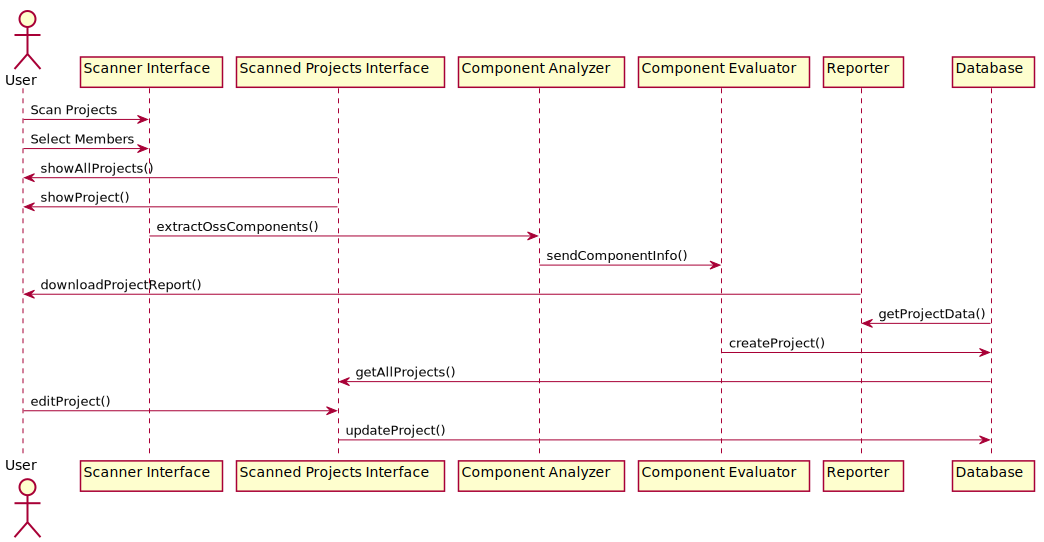
\includegraphics[width=15cm]{includes/sequence_diagram.png}
	\centering
	\caption{\acs{OSS} scanner sequence diagram}
	\label{fig:sequence}
\end{figure} 
\subsection{Scanner Components}

As shown in figure ~\ref{fig:architecture} there are three main components involved in the design and architecture of the \acs{OSS} scanner. Following are the components which are inter related to each other and gives a big picture of their functionality. \acs{OSS} Component Analyzer, \acs{OSS} Component Evaluator and \acs{OSS} Reporter.

\textbf{\acs{OSS} Component Analyzer:} This component is mainly responsible for extracting the \acs{OSS} components used in the projects. This particular task should be performed on the client side where the scanning should take place in the browser. The inputs required in this interface by the user are Project name, description, members and project directory. After receiving the inputs, there are two stages of the automation process, first the scanner will detect what type of application framework is given as input so that the scanner can parse the targeted file for the further process. Once the target file is parsed, the second process will extract the \acs{OSS} component name and the version used in the project. It creates \acs{JSON} data with basic project information along with the list of \acs{OSS} components and its version. Overall the primary goal of this component is to extract all the \acs{OSS} components and It will send the data evaluation process.
	
\textbf{\acs{OSS} Component Evaluator:} This component evaluates the \acs{OSS} components which are extracted by the analyzer. The evaluation process component will be developed as a back-end application so that the process will be performed on the server side. This evaluation is performed with the help of \acs{NVD} database \acs{API} service. The extracted \acs{OSS} components will be searched in the \acs{NVD} database by using its name and version to find the known vulnerabilities registered under the respective component version. This component will be running asynchronously in the server because a project can have n-number of \acs{OSS} components. Once the \acs{OSS} components are evaluated, the information which is collected from the \acs{NVD} database is used for analysing the risk level of each \acs{OSS} component. Finally all the information is converted as a \acs{JSON} file and stored as container in Azure data storage.
	
\textbf{\acs{OSS} Reporter:} This component is a part of the scanner’s user interface where the user can download the \acs{OSS} report of the project. This report shows all the basic information of the project and its \acs{OSS} component along with the vulnerability and the risk level of each component. This component simply generates a pdf report with all the above information retrieved from the database.
	
\subsection{Design Challenge}
Almost every software product development project has a unique set of problems. These issues can be a roadblock to development throughout system design and, more importantly, during implementation. There were several difficulties faced throughout the implementation of this thesis. The major problems that need to be addressed and a solution formed are listed below.

\textbf{Application framework:} Because I had never worked with Angular framework before, the first hurdle I had while starting implementation was familiarizing myself with it. I got acquainted to the Angular environment with the aid of several online tutorials and hands-on programming. The are few reasons why we chose to develop frontend application with  Angular framework because it has faster development process like having neat documentation for understanding Angular with a large developer community and it also helps us with efficient problem-solving patterns where the angular services helps to integrate the business logic with app user-interface.
	
\textbf{File structure:} The next challenge for me was trying to create a generic function that can extract the \acs{OSS} component name version from respected config files of the software project. This challenge was pretty time consuming because each software project can be built by using a different application framework and also each application framework has its own dependency manager. For instance, the Ruby on Rails application framework uses RubyGems as a dependency manager. The Ruby on Rails application framework generates file called Gemfile where all the required dependencies of the project will be mentioned there along with the version of the dependency. The file type of the the Gemfile is .gemfile.  Likewise each application framework have different file type as refereed in the table ~\ref{tab:configFiles}. To over come this challenge, when the project data is submitted at the beginning, the project data should pass a condition where it has to identify which application framework project it is. Once after identifying the application, the OSS component extraction will be performed based on the file type of config file. So for each application framework, there should be different extraction functions. 
	
	
\textbf{Finding the right regex:} Another challenge was finding the right regex for each config file. The harder part was extracting the \acs{OSS} component names and version from config files like Gemfile and requirements.txt. To overcome this challenge it was not that difficult because the same solution like file structure is required for the this challenge. When the user submits a Django or Ruby on Rails project, firstly as I said the condition will identify the application framework and based on the file type the extraction will be performed. The regex is implemented in the extraction function, for instance when you see the figure ~\ref{fig:ruby} which lists all the OSS components used in a Ruby on Rails project. Each line of the file will be sent for a cleaning process and delivers the component name and version which is extracted from each line. To extract the name and version from each line a proper regex is required. Like the Django and Ruby on Rails, the other application framework was no that difficult because most of the file types were xml and json files where the component name version can be easily extracted with the help of json and xml DOM parsing functions.  
	
\textbf{Verification:} Another issue was determining whether what I built corresponded to what was actually happening within the software. To do so, I ran my code on a set of test inputs to check if the program produced the same results. At the beginning, the results were not coming as expected, for instance the results will come without the component name or its version. This happens due to faulty regex commands, so it required lot of testing with many set of inputs to improve the extraction. There is another challenge where a same application framework can have different config files based on the type of the project. This challenge was with .Net projects because for each type of project it has different config file like stated in the table ~\ref{tab:configFiles}. So to overcome this challenge, only the .Net based projects has to pass multiple condition to identify in which type of project it belongs in .Net application framework.

%

%
\newpage
%
\section{Implementation}\label{sec:implementation}
This chapter explains how the component is developed. The ways to overcome the design challenges, some of the findings during the development have been written down.
%
\subsection{System Characteristics}
When beginning the implementation, I decided to use a simple yet powerful programming language for both frontend and backend applications to obtain my results. The programing languages which I selected was javascript for frontend and C\# for the backend. To simplify my programming work, I used the Visual Studio Code IDE for the frontend and Visual Studio 2019 for the backend. The configuration of the computer used for implementation is as follows:
\begin{description}
	\item [$\bullet$]Operating System: Windows 10 Enterprise 2016 - 64-bit
	\item [$\bullet$]Processor: Intel Core i7-6700 @ 3.4GHz
	\item [$\bullet$]RAM: 16GB
	\item [$\bullet$]HDD: 500GB
\end{description}

The software support tools used for frontend implementation are listed as follows:
\begin{description}
	\item [$\bullet$]Programming Language: Javascript
	\item [$\bullet$]IDE: Visual Studio Code
	\item [$\bullet$]Packet Manager: npm
	\item [$\bullet$]Version Control: Azure Repos
\end{description}

The software support tools used for backend implementation are listed as follows:
\begin{description}
	\item [$\bullet$]Programming Language: C\#
	\item [$\bullet$]IDE: Visual Studio 2019
	\item [$\bullet$]Packet Manager: NuGet
	\item [$\bullet$]Database: Azure Data Storage - Containers
	\item [$\bullet$]Version Control: Azure Repos
\end{description}

All the infrastructure and software that I used are provided by evosoft GmbH.
\subsection{OSS Component Analyzer}

\subsection{Component Evaluator}

\subsection{Reporter}
%

%
\newpage
%
\section{Results \& Discussion}\label{sec:Results & Discussion}
%
This is the last chapter of this thesis \cite{tur38}.
%

%
\newpage
%
\section{Conclusion \& Future Work}\label{sec:conclusion}

\subsection{Conclusion}
In this thesis, we have focused on automating the open-source software discovery by developing a client-side scanner and finding a suitable vulnerability database to find the \acs{OSS} component’s vulnerability. Software security is one of the most significant quality assurance measures for software. It has been shown that software security is one of the most critical and essential parts to focus on before the application gets delivered to the end user[4]. This proposed scanner is developed to find all the OSS components used in a software project, and this solution will help the developers to find the vulnerabilities present in the \acs{OSS} component. The scanner can scan the following application framework projects: Django, Laravel, Ruby on Rails, .Net core, Gradle and Maven.

This implementation has the advantage that the \acs{OSS} component analyzer module can be reused for integrating with another vulnerability database. Also, it can be modified by adding a new application framework project for scanning. The end report provided by the system will not take or suggest any decisions on behalf of the user. The report will give the vulnerability findings of each component where the developer can decide whether to keep the same version or move to a different version of the \acs{OSS} component. This thesis implementation will be helpful for the first level of security check before delivering the application to the end-user.

\subsection{Future Work}
Our work shows a direction for further development and research in the domain of open-source software security. We have developed a scanner that extracts the \acs{OSS} components from software projects with the help of dependency managers. There are numerous
possibilities to improve or customize this scanner according to the application scenario.

The extracted \acs{OSS} component from the software projects can be used for creating a license clearing tool. The license clearing tool is another crucial process in an organization to maintain transparency towards software usage. If the license is adequately maintained, then the organization can avoid the unwanted cost e.g. copyleft issues \cite{copyleft}.

Apart from automating the extraction of \acs{OSS} components and delivering the vulnerability information of each \acs{OSS} component, we can also develop an extra feature like recommending the nearest version with less vulnerability of the same component. In this case, the user can have an idea of the nearest version of the component.

There could be many other ways to improve the scanner, other than the ones pointed out by us. However, we believe that the scanner so far has yielded satisfactory results, as is evident from the evaluation. We hope to see more improvements in this scanner, or in general, in the field of open-source software security.
%
%
%\newpage
%%
\section{Future Work}\label{sec:future_work}
%
This is the last chapter of this thesis \cite{tur38}.
%

%
\newpage
%
% References
\addcontentsline{toc}{section}{References}
\bibliographystyle{alpha}
%
% Insert your bibliography here
\bibliography{bibliography/references}
\newpage
%
% Eigenständigkeitserklärung APO
\makedeclaration{master’s thesis}{23.09.2021}{Hari Prashanth Rajendran}
%
\end{document}
